% !TEX TS-program = pdflatex
% !TEX encoding = UTF-8 Unicode

% This is a simple template for a LaTeX document using the "article" class.
% See "book", "report", "letter" for other types of document.

\documentclass[11pt]{article} % use larger type; default would be 10pt

\usepackage[utf8]{inputenc} % set input encoding (not needed with XeLaTeX)

%%% Examples of Article customizations
% These packages are optional, depending whether you want the features they provide.
% See the LaTeX Companion or other references for full information.

%%% PAGE DIMENSIONS
\usepackage{geometry} % to change the page dimensions
\geometry{a4paper} % or letterpaper (US) or a5paper or....
% \geometry{margin=2in} % for example, change the margins to 2 inches all round
% \geometry{landscape} % set up the page for landscape
%   read geometry.pdf for detailed page layout information

\usepackage{graphicx} % support the \includegraphics command and options

% \usepackage[parfill]{parskip} % Activate to begin paragraphs with an empty line rather than an indent

%%% PACKAGES
\usepackage{booktabs} % for much better looking tables
\usepackage{array} % for better arrays (eg matrices) in maths
\usepackage{paralist} % very flexible & customisable lists (eg. enumerate/itemize, etc.)
\usepackage{verbatim} % adds environment for commenting out blocks of text & for better verbatim
\usepackage{subfig} % make it possible to include more than one captioned figure/table in a single float
\usepackage{amsmath}

% These packages are all incorporated in the memoir class to one degree or another...

%%% HEADERS & FOOTERS
\usepackage{fancyhdr} % This should be set AFTER setting up the page geometry
\pagestyle{fancy} % options: empty , plain , fancy
\renewcommand{\headrulewidth}{0pt} % customise the layout...
\lhead{}\chead{}\rhead{}
\lfoot{}\cfoot{\thepage}\rfoot{}

%%% SECTION TITLE APPEARANCE
\usepackage{sectsty}
\allsectionsfont{\sffamily\mdseries\upshape} % (See the fntguide.pdf for font help)
% (This matches ConTeXt defaults)

%%% ToC (table of contents) APPEARANCE
\usepackage[nottoc,notlof,notlot]{tocbibind} % Put the bibliography in the ToC
\usepackage[titles,subfigure]{tocloft} % Alter the style of the Table of Contents
\renewcommand{\cftsecfont}{\rmfamily\mdseries\upshape}
\renewcommand{\cftsecpagefont}{\rmfamily\mdseries\upshape} % No bold!

%
%%%%% Packages used to loop through the list
%
\usepackage{etoolbox}
%
% Defining some useful macros
%

\def \beg {\begin{equation}}
\def \en {\end{equation}}
 
\def\ece#1#2{
	\expandafter#1\csname#2\endcsname
}%

\def\setproperty#1#2#3{%
	\ece \edef{#1@p#2}{#3}
}%
\def\setpropertyglobal#1#2#3{\ece\protected@xdef{#1@p#2}{#3}}%

\def\getproperty#1#2{%
  \expandafter\ifx\csname#1@p#2\endcsname\relax
  % then \empty
  \else \csname#1@p#2\endcsname
  \fi
}%

\def \printmylist#1{% have a way of looping through the list
	\dolistloop{#1}
}


%
% Match the #1 symbol and then use
% the #2 string to find possible derivatives
% 
%\def\create_derivative#1#2{	
%}
%
%Macros that are needed to write down the equations
%

\def \1/r {\frac{1}{r}}


%%% END Article customizations

%%% The "real" document content comes below...

\title{HypoElastic Models}
\author{Sumanta Mukherjee}
%\date{} % Activate to display a given date or no date (if empty),
         % otherwise the current date is printed 

\begin{document}
%%%%%%%%%%%%%%%%%%%%%%%%%%%%%%%%%%%%%%%%%%
%macros property
%

%\documentclass{article}
%\usepackage{etoolbox}
%\usepackage{amsmath}

\newcommand{\addwithcounting}[3]{%
	\stepcounter{#1}
	\listadd{#2}{#3}
}


\newcommand\printItem[3]{

	\stepcounter{innercounter}

	\ifnumless{\value{innercounter}}{\value{columncounter}}{%
		#1_{#2#3} &
	}{%
		#1_{#2#3}% Final column, do not add a & character
	}% 
}

\newcommand\createMatrix[3]{%
	\begin{pmatrix}
		\getOuterLoop{#2}{#3}{#1}
	\end{pmatrix}
}
	
\newcommand\getOuterLoop[3]{%
	 % #1 row list #2 column list
	\forlistloop{\setcounter{innercounter}{0}\getInnerLoop{#3}{#1}}{#2}
}

\newcommand\getInnerLoop[3]{%
	\forlistloop{\printItem{#1}{#3}}{#2} \\
}

%\newcommand\printItemContracted[4]{
%	
%	\stepcounter{innercounter}
%	
%	\ifnumless{\value{innercounter}}{\value{columncounter}}{%
%		#1_{#3#4}#2_{#3#4} + 
%	}{%
%		#1_{#3#4}#2_{#3#4}% Final column, do not add a & character
%	}% 
%}


%\newcommand\ContractedProduct[2]{% 
%	\forlistloop{\setcounter{innercounter}{0}\getOuterLoopContracted{\sigma}{\epsilon}{#1}}{#2}
%}

%\newcommand{\getOuterLoopContracted}[4]{%
%	\forlistloop{\printItemContracted#1#2#3}{#4}
%}

\newcommand{\showlist}[1]{
	#1
}
\newcommand{\ContractedProduct}[2]{%
	  \begin{pmatrix}
		\setcounter{outercounter}{0}
		\forlistloop{\grabfromouterlist{\sigma}{\epsilon}{#1}}{#2} 
	\end{pmatrix} dr dz
}

\newcommand{\grabfromouterlist}[4]{%
	%
	\setcounter{innercounter}{0}% Reset the inner counter
	\stepcounter{outercounter}%
	%
	\ifnumless{\value{outercounter}}{\value{rowcounter}} {		
		\forlistloop{\grabfrominnerlist{#1}{#2}{#4}}{#3} +
	}{%
		\forlistloop{\grabfrominnerlist{#1}{#2}{#4}}{#3}
	}%
	  % use the 2nd argument which is fed from the outer loop actually and process the list given as 1st argument. 
}

\newcommand{\grabfrominnerlist}[4]{%
	\stepcounter{innercounter}%
	\ifnumless{\value{innercounter}}{\value{columncounter}}{%
		#1_{#3#4}#2_{#3#4} + % typeset the matrix element with index of row and column number
	}{%
		#1_{#3#4}#2_{#3#4}  % Final column, do not add a & character
	}%
}



%\begin{document}	
%	\newcounter{rowcounter}
%	\newcounter{columncounter}
%	\newcounter{innercounter}
%	
%	\setcounter{rowcounter}{0}
%	\setcounter{columncounter}{0}
%
%	\def\mycolumnlist{}  
%	\def\myrowlist{}  
%	
%	\forcsvlist{\addwithcounting{rowcounter}{\myrowlist}}{r,\theta,z}
%	\forcsvlist{\addwithcounting{columncounter}{\mycolumnlist}}{r,\theta,z}
%
%	
%	\createMatrix{\sigma}{\myrowlist}{\mycolumnlist} :  %\createMatrix{\sigma}{\myrowlist}{\mycolumnlist}
%	\ContractedProduct{\myrowlist}{\mycolumnlist}
%	 
%\end{document}

\def\set_prop#1#2#3 {% first paramenter is layer number, 
				%second parameter is r, b, c
	\setproperty{sigma_prime_coeff}{#1}{
		\frac{ ({#3}^{2} - {#2}^{2}) } {2 {r}}
	}
}

\def\get_prop#1 {
	\getproperty{sigma_prime_coeff}{#1}
}

\setproperty{sigma_prime_coeff}{1}{
	\frac{ ({a}^{2} - {r}^{2}) } {2 r}
}
\setproperty{sigma_prime_coeff}{2}{
	\frac{ ({b}^{2} - {r}^{2}) } {2 r}
}
\setproperty{sigma_prime_coeff}{3}{
	\frac{ ({c}^{2} - {r}^{2}) } {2 r}
}

\setproperty{sigma}{1}{
	\sigma^{'(1)}\getproperty{sigma_prime_coeff}{1}
}

\setproperty{sigma}{2}{
	\sigma^{'(2)}\frac{ ({b}^{2} - {r}^{2}) } {2 r} + \sigma^{'(1)}\frac{ ({a}^{2} - {b}^{2}) } {2 r}
}

\setproperty{sigma}{3}{
	\sigma^{'(3)}\frac{ ({c}^{2} - {r}^{2}) } {2 r} + \sigma^{'(2)}\frac{ ({b}^{2} - {c}^{2}) } {2 r} + \sigma^{'(1)}\frac{ ({a}^{2} - {b}^{2}) } {2 r}
} 

\setproperty{sigma_coeff}{v1}{
	\frac{(b^2 -a^2)}{(c^{2} - d^{2})}
}

\setproperty{sigma_coeff}{v2}{
	\frac{(c^2 -b^2)}{(c^{2} - d^{2})}
}

\setproperty{sigma_2_prime_coeff}{v1} {
	\Bigg({\frac {a^{2} ln{(r/a)}}{2} -\frac{(a^2 - r^2)}{2.2} } \Bigg)
}

\setproperty{sigma_2_prime_coeff}{v2} {
	\Bigg({\frac {b^{2} ln{(r/b)}}{2} -\frac{(b^2 - r^2)}{2.2} } \Bigg)	
}

\setproperty{sigma_2_prime_coeff}{v3} {
	\Bigg({\frac {c^{2} ln{(r/c)}}{2} -\frac{(c^2 - r^2)}{2.2}} \Bigg)		
}

\setproperty{sigma3_2_prime}{v3}{
	\Bigg(
	\sigma^{''(1)}\getproperty{sigma_coeff}{v1} + \sigma^{''(2)}\getproperty{sigma_coeff}{v2}
	\Bigg)
}

%%%%%%%%%%%%%%%%%%%%%%%%%%%%%%%%%%%%%%%%

\long\def\for#1in#2#3{
	\expandafter\def\csname b:\string#1\endcsname{#3}%
	\forinA#1#2,,
}

\def\forinA#1#2,{
	\ifx,#2,\else
		\def#1{#2}\csname b:\string#1\endcsname \expandafter
	\forinA\expandafter#1\fi
}



\maketitle

\section{The differential equation for a Tubular Structure}

Hypoelastic Materials are important in everyday life. Below we create the mathematical framework for hypoelastic material which is an adhesive between two linear elastic materials.


\subsection{The basic equations}

%\[
	\begin{equation}
	\nabla \cdot \sigma  = 0 
	\end{equation}

	\begin{equation}
	\epsilon = \frac{1}{2}((\nabla u) + (\nabla u)^T)
	\end{equation}

	\begin{equation}
	\epsilon_{ij} = \alpha_1{\sigma_{ij}} - \alpha_2 {\sigma_{kk}} \delta_{ij} + \alpha_3 S_{ij}(\frac{\sigma_{eq}}{\sigma_{0}})^{(n-1)}
	\end{equation}

	\begin{figure}[htp] \centering{
	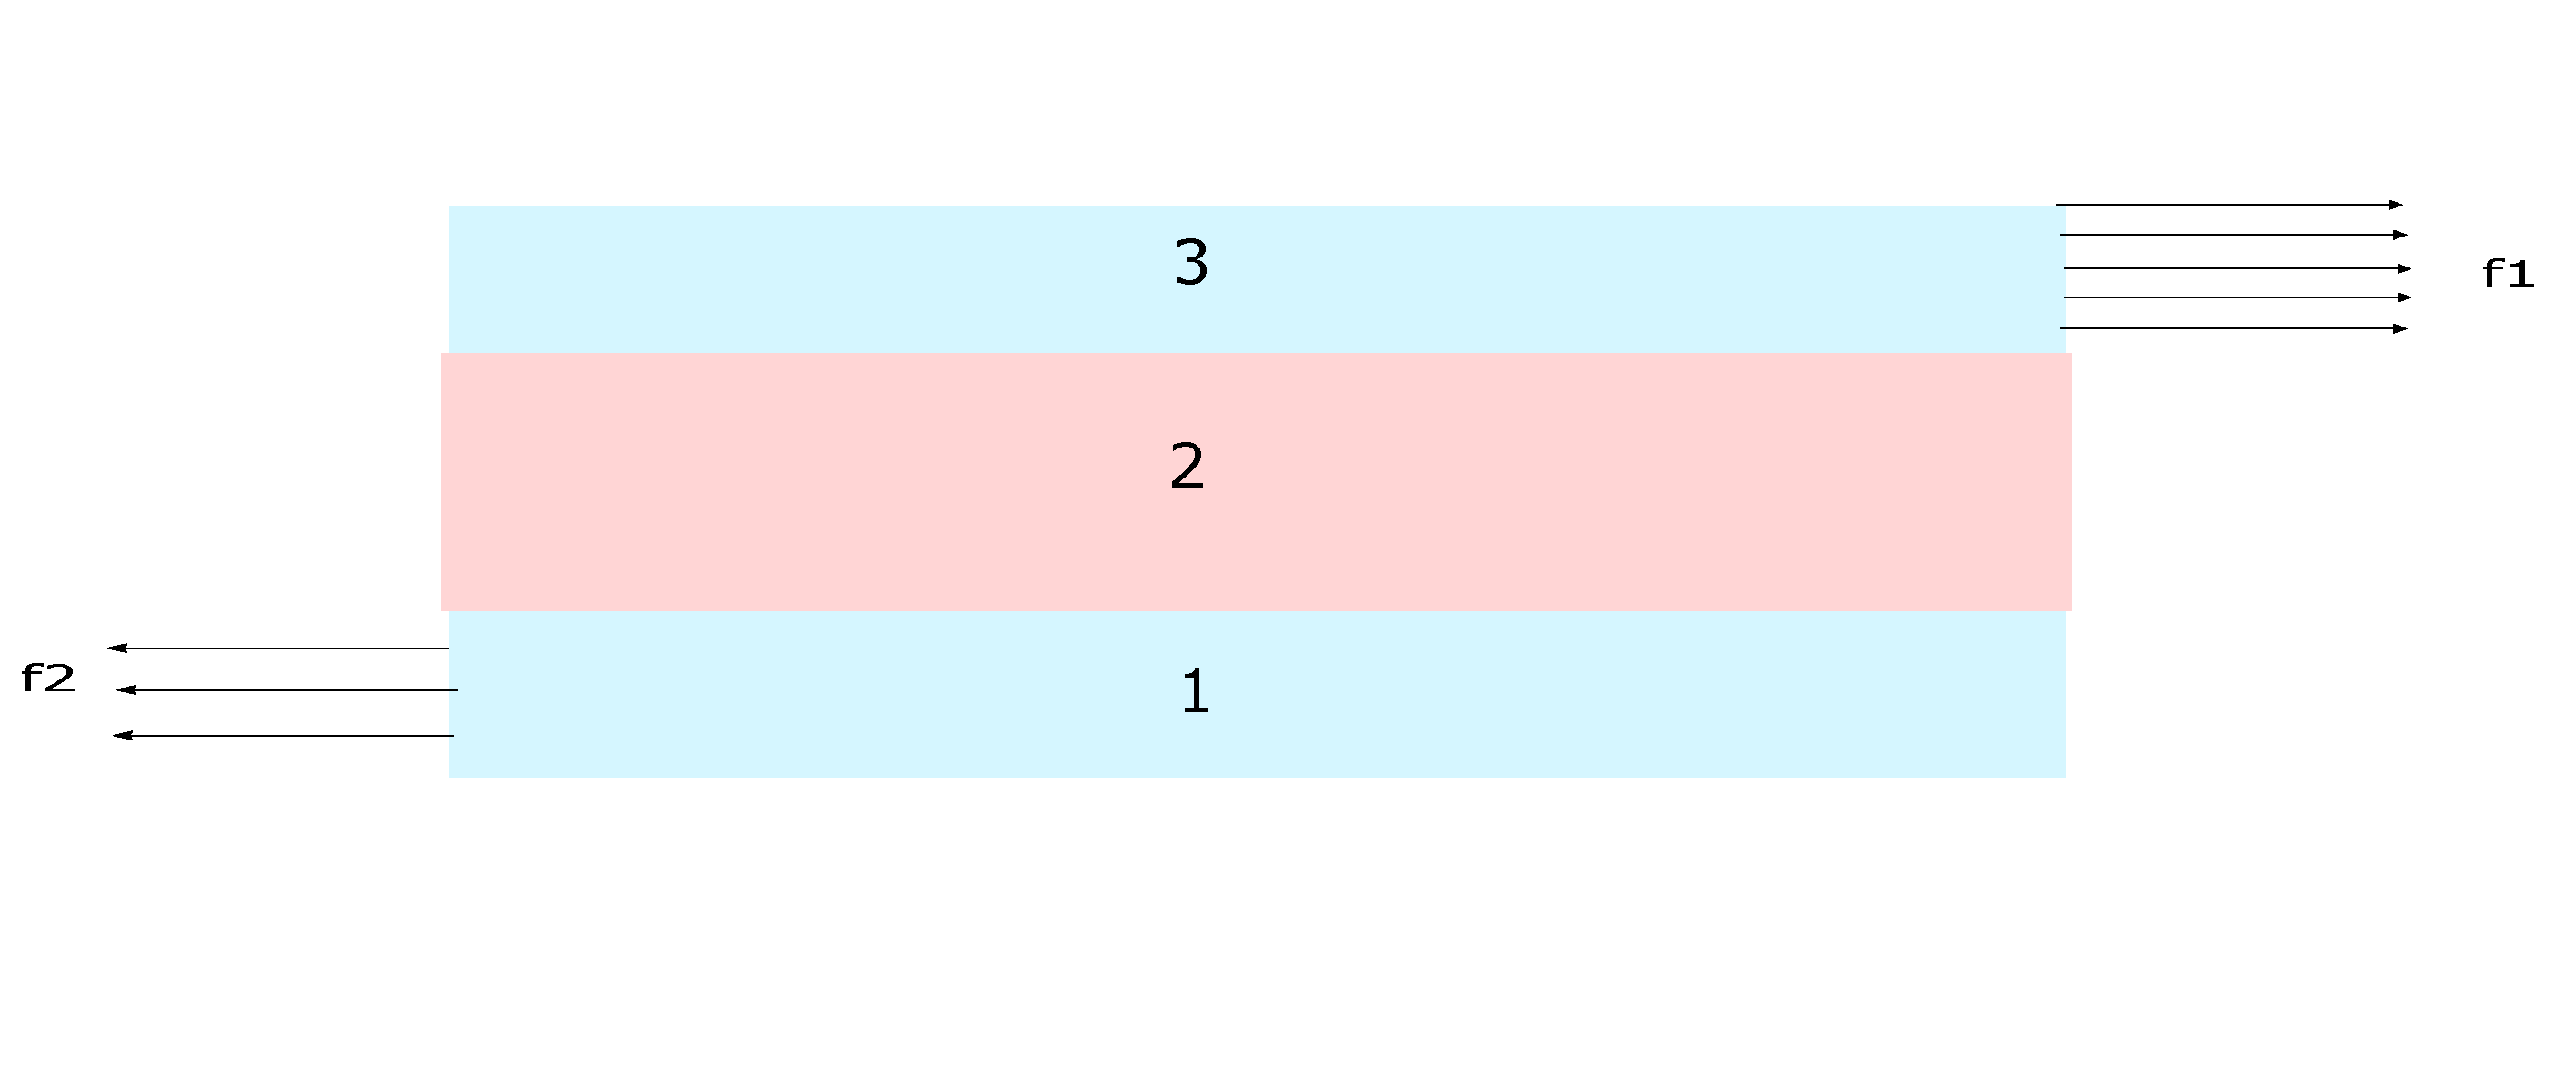
\includegraphics[scale=0.25]{drawing-1.pdf}}
	\caption{}
	\end{figure}

	The three layers are marked 1,2, 3. The blue layers are made up of linear elastic material while the intermediate adhesive layer is made up of hypoelastic material. 
	
	The expanded equations for one of the tubular structure in $ r , \theta, z $ direction is given as follows.
	
	\beg
		\begin{aligned}
			\frac{\partial \sigma_{rr}}{\partial r} + \frac {\sigma_{rr} - \sigma_{\theta\theta}}{r} + 
					\1/r \frac{\partial \sigma_{r\theta}}{\partial \theta} + 
					\frac{\partial \sigma_{rz}}{\partial z}  & =  &  0 \\
			\frac{\partial \sigma_{r\theta}}{\partial r} + \frac {2\sigma_{r\theta}}{r} + 
					\1/r \frac{\partial \sigma_{\theta\theta}}{ \partial \theta} + 
					\frac{\partial \sigma_{\theta z}}{\partial z}  & = & 0 \\
			\frac{\partial \sigma_{rz}}{\partial r} + \frac {\sigma_{rz}}{r} + 
					\1/r \frac{\partial \sigma_{z\theta}}{ \partial \theta} + 
					\frac{\partial \sigma_{zz}}{\partial z} & = & 0
		\end{aligned}
	\en
		

	The expanded equations for the cylindrical geometry of the multilayer tubular structure are subject to the following assumptions.
	\begin{itemize}
		\item The radial stresses are directly proportiional to the hoop stresses in all the three domains
		\item Axisymmetric condition implies that only the shear stress $\sigma_{rz}$ is non zero in all the three domains.
		\item variations with respect to $\theta$ is also insignificant
	\end{itemize}

	The equations therefore reduce to the following form.
	\beg
		\begin{aligned}
			 \frac{1}{r}\frac{\partial(r\sigma_{rr}^{(i)})}{\partial r} + \frac {- \sigma_{\theta\theta}}{r} +  
					\frac{\partial \sigma_{rz}}{\partial z}  & =  &  0 \\
			\frac{\partial \sigma_{rz}}{\partial r} + \frac {\sigma_{rz}}{r} +  
					\frac{\partial \sigma_{zz}}{\partial z} & = & 0
		\end{aligned}
	\en

There are 3 unknowns from two equations and so a relation needs to be found out between the stresses $ \sigma_{\theta\theta}, \sigma_{rz}, \sigma_{zz} $.

We describe the force balance in each of the layers

Layer  i = 1,3: (Linear Elastic Material Layer)
		\beg
		\begin{aligned}
			\frac{1}{r}\frac{\partial(r\sigma_{rr}^{(i)})}{\partial r} + \frac {- \sigma_{\theta\theta}^{(i)}}{r} +  
					\frac{\partial \sigma_{rz}^{(i)}}{\partial z}  & =  &  0 \\
			\frac{\partial \sigma_{rz}^{(i)}}{\partial r} + \frac {\sigma_{rz}^{(i)}}{r} +  
					\frac{\partial \sigma_{zz}^{(i)}}{\partial z} & = & 0
		\end{aligned}
		\en

Layer 2: (Adhesive Hypo Elastic Material Layer)
		\beg
		\begin{aligned}
			\frac{1}{r}\frac{\partial(r\sigma_{rr}^{(2)})}{\partial r} + \frac {- \sigma_{\theta\theta}^{(2)}}{r} +  
					\frac{\partial \sigma_{rz}^{(2)}}{\partial z}  & =  &  0 \\
			\frac{\partial \sigma_{rz}^{(2)}}{\partial r} + \frac {\sigma_{rz}^{(2)}}{r} +  
					\frac{\partial \sigma_{zz}^{(2)}}{\partial z} & = & 0
		\end{aligned}
		\en

Solving the equations and using the notation $ \frac{\partial \sigma_{zz}}{\partial z}  = \sigma^{'}$  with the boundary condition $ \sigma_{rz} (a) = 0 $ we come to the following solution of the equation
	\beg
	\frac{1}{r}\frac{\partial (r\sigma_{rz})}{\partial r} +  \sigma^{'}   = 0
	\en

as 
	\beg
		\begin{aligned}
			\frac{\partial (r\sigma_{rz})}{\partial r} = -\sigma^{'}{r} \\
			r\sigma_{rz} =  -0.5 \sigma^{'}{r}^{2} + const 
		\end{aligned}
	\en
	Applying the Boundary Condition in the first region 
	\beg
		\begin{aligned}
			0.5 \sigma^{'}{a}^{2} =  const 
		\end{aligned}
	\en
	Applying the Boundary Condition in the second region 
	\beg
		\begin{aligned}
			0.5 \sigma^{'(1)}({a}^{2} - {b}^{2}) + 0.5 \sigma ^{'(2)}({b}^{2}) =  const 
		\end{aligned}
	\en
	Applying the Boundary Condition in the third region 
	\beg
		\begin{aligned}
			0.5 \sigma^{'(1)}({a}^{2} - {b}^{2}) + 0.5 \sigma ^{'(2)}({b}^{2} - {c}^{2}) + 0.5 \sigma ^{'(3)}({c}^2)=  const  
		\end{aligned}
	\en

	Substituting the solution into the first of the two equations for each of the regions and making the assumption that  $ \sigma_{\theta\theta} = \sigma_{rr}$


	\beg
		\boxed{
		\begin{aligned}
			\sigma_{rz}^{(1)} & = \getproperty{sigma}{1}\\
			\sigma_{rz}^{(2)} & = \getproperty{sigma}{2} \\ 
			\sigma_{rz}^{(3)} & = \getproperty{sigma}{3}
		\end{aligned}
		}
	\en		

	Given that the stress on the outside is also zero we get the following condition.
	\beg
		\boxed {
			\sigma^{'(3)}({c}^{2} - {d}^{2})  + \sigma^{'(2)}({b}^{2} - {c}^{2})  +  \sigma^{'(1)}({a}^{2} - {b}^{2})  = 0
		}
	\en

%
% Now one needs to use the above equations and find out the radial stresses in each of the three layers
%

	The first equation is therefore with $\sigma_{\theta\theta} = \sigma_{rr}$ in each of the layers
	\beg
		\begin{aligned}
			\frac{1}{r}\frac{\partial(r\sigma_{rr})}{\partial r} + \frac {- \sigma_{rr}}{r} +   
					\frac{\partial \sigma_{rz}}{\partial z}  & =  &  0 
		\end{aligned}
	\en
	This is equal to the following after substituting for the value of  $\sigma_{rz} $ and application of the boundary conditions in each of the regions 
	\beg		
		\boxed{
			\begin{aligned}
				\sigma_{rr}^{(1)} & = \sigma^{''(1)}\Bigg({\frac {a^{2} ln{(r/a)}}{2} - \frac{(a^2 - r^2)}{2.2} } \Bigg)\\
%					
				\sigma_{rr}^{(2)} & = \sigma^{''(2)}\Bigg({\frac {b^{2} ln{(r/b)}}{2} - \frac{(b^2 - r^2)}{2.2} } \Bigg) + 		\Bigg(\sigma^{''(1)}\frac{(a^{2} -b^{2})}{2} ln(r/b) \Bigg)\\ 
%					
				\sigma_{rr}^{(3)} & = \sigma^{''(3)}\Bigg({\frac {c^{2} ln{(r/c)}}{2} - \frac{(c^2 - r^2)}{2.2} } \Bigg)  + 		\Bigg(\sigma^{''(2)}\frac{(b^{2} -c^{2})}{2} ln(r/c) \Bigg) +\Bigg(\sigma^{''(1)}\frac{(a^{2} -b^{2})}{2} ln(r/c) \Bigg)   
			\end{aligned}	
		}
	\en

	Now for the model of $\sigma^{'(i)} $ in the different layers.
	Making a force balance along the z direction we get the following

	
%	\setproperty{sigma_prime}{v1}{\sigma{''}\getproperty{sigma_coeff}{v1} + \sigma{(1)''}\getproperty{sigma_coeff}{v2}} 

	\beg
		\begin{aligned}
			f_1(b^{2} - a^{2}) = f_2(d^{2} - c^{2}) = \sigma_{zz}^{(1)}(b^{2} - a^{2}) +  \\
				\sigma_{zz}^{(2)}(c^{2} - b^{2}) + \sigma_{zz}^{(3)}(d^2 - c^2) \\
		%
		%
			\sigma_{zz}^{(3)} = f_2 + \sigma_{zz}^{(1)}\getproperty{sigma_coeff}{v1} + \sigma_{zz}^{(2)} \getproperty{sigma_coeff}{v2}					 
		\end{aligned}		
	\en

	Thus substituting the values we get the following two parameter model based on $\sigma^{'(1)} \text{ and } \sigma^{'(2)} $
	
		
	\beg
		\boxed {
			\begin{aligned}
				%
				\sigma_{rr}^{(1)} & = \sigma^{''(1)}\getproperty{sigma_2_prime_coeff}{v1}\\
				%
				%
				\sigma_{rr}^{(2)} & = \sigma^{''(2)}\getproperty{sigma_2_prime_coeff}{v2} + \sigma^{''(1)}\Bigg(\frac{(a^{2} -b^{2})}{2} ln(r/b) \Bigg)\\
				%
				%
				\sigma_{rr}^{(3)} &  = \sigma^{''(3)}\getproperty{sigma_2_prime_coeff}{v3}+
				\sigma^{''(2)}\Bigg(\frac{(b^{2} -a^{2})}{2} ln(r/c)\Bigg) + 
				\sigma^{''(1)}\Bigg(\frac{(a^{2} -b^{2})}{2} ln(r/b)\Bigg) \\
				%
				%
				& = \getproperty{sigma3_2_prime}{v3}
				\getproperty{sigma_2_prime_coeff}{v3} + 
				\sigma^{''(2)}\Bigg(\frac{(b^{2} -a^{2})}{2} ln(r/c)\Bigg) + 
				\sigma^{''(1)}\Bigg(\frac{(a^{2} -b^{2})}{2} ln(r/b)\Bigg) \\
				%\getproperty{test}{aproperty}
			\end{aligned}
		} 		
	\en

Now substituting the values for the $\sigma_{rz}^{(i)} $ we can see the following 

	\beg
		\set_prop{1}{b}{a}
		\set_prop{2}{c}{b}
		%
		\boxed {
		\begin{aligned}
			\sigma_{rz}^{(1)} & = \getproperty{sigma}{1}\\
			\sigma_{rz}^{(2)} & = \getproperty{sigma}{2} \\ 
			\sigma_{rz}^{(3)} & = \getproperty{sigma}{3} \\
			& = \Big( 
					\sigma^{'(1)}\getproperty{sigma_coeff}{v1} +
					\sigma^{'(2)}\getproperty{sigma_coeff}{v2} 
				\Big)(\getproperty{sigma_prime_coeff}{3}) + \sigma^{'(2)}\get_prop{2} +
				\sigma^{'(1)}\get_prop{1}
		\end{aligned}
		} 		
	\en
	
	The energy of the system that is there needs to be minimized in this case and therefore the overall energy density in the three layers are given for each of the layers
	

	\newcounter{rowcounter}
	\newcounter{columncounter}
	\newcounter{innercounter}
	\newcounter{outercounter}
	%	
	\setcounter{rowcounter}{0}
	\setcounter{columncounter}{0}
	%
	\def\mycolumnlist{}  
	\def\myrowlist{}  
	%	
	\forcsvlist{\addwithcounting{rowcounter}{\myrowlist}}{r,\theta,z}
	\forcsvlist{\addwithcounting{columncounter}{\mycolumnlist}}{r,\theta,z}

	$
		E = \int_{0}^{r}\int_{0}^{L}
		\createMatrix{\sigma}{\myrowlist}{\mycolumnlist} :  \createMatrix{\epsilon}{\myrowlist}{\mycolumnlist} dr dz
	$ 
		 
	
	$ 
		E = \int_{0}^{r}\int_{0}^{L}\ContractedProduct{\myrowlist}{\mycolumnlist}
	$	
\end{document}
